\subsection{Message Broker}
\label{s_message_broker}

% Introduction {{{
A message broker is an intermediary computer program module
that translates a message from the formal messaging
protocol of the sender to the formal messaging protocol of
the receiver.

Message brokers are elements in telecommunication or
computer networks where software applications communicate
by exchanging formally-defined messages. Message brokers
are a building block of message-oriented middleware (MOM)
but are typically not a replacement for traditional
middleware like MOM and remote procedure call (RPC).
\cite{amjad27}
% }}}

% History {{{
\subsubsection{History}

Message broker products are the middleware that embody
different messaging solutions. In 1983 Vivek Ranadivé from
Teknekron Software Systems began working on an idea based
on the ideals of a Software Bus to enable applications to
share data in a standard fashion. That work would later be
referred to as “The Information Bus”. Already in 1986 his
ideas were put to use when Goldman Sachs, an American
investment banking firm, launched cooperation with
Teknekron to find solutions for the trading floor of the
future.\cite{amjad28}

For nearly two decades the domain of message exchange was
left for proprietary vendors and proprietary formats.
Throughout the 1980s and 1990s message queuing kept
evolving but in isolation since commercial message queue
vendors strived for interoperability between client
applications rather than worked on standardized interfaces
for their message queuing products to utilize.
\cite{amjad28}


The figure bellow shows a brief timeline of message queuing:

\begin{figure}[H]
  \centering
  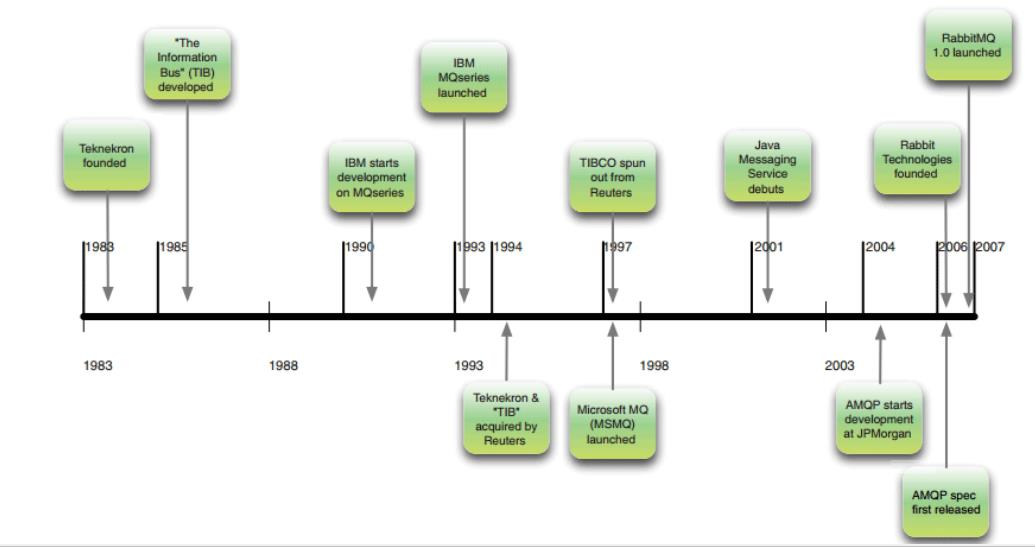
\includegraphics[width=\linewidth]{%
    diagrams/messaging_history.png}
  \caption{Timeline of message queuing}
\end{figure}
% }}}

% Functionality and architecture {{{
\subsubsection{Functionality and architecture}
\label{ss_mb_faa}

A message broker is an architectural pattern for message
validation, transformation, and routing.

It mediates communication among applications, minimizing
the mutual awareness that applications should have of each
other in order to be able to exchange messages, effectively
implementing decoupling.\cite{amjad29}

The primary purpose of a broker is to take incoming
messages from applications and perform some action on them.
Message brokers can decouple endpoints, meet specific non-
functional requirements, and facilitate reuse of
intermediary functions. For example, a message broker may
be used to manage a workload queue or message queue for
multiple receivers, providing reliable storage, guaranteed
message delivery and perhaps transaction management.
\cite{amjad27}

Message brokers are generally based on one of two
fundamental architectures: hub-and-spoke and message bus.
In the prior, a central server acts as the mechanism that
provides integration services, whereas with the latter, the
message broker is a communication backbone or distributed
service that acts on the bus.\cite{amjad30}

\begin{figure}[H]
  \centering
  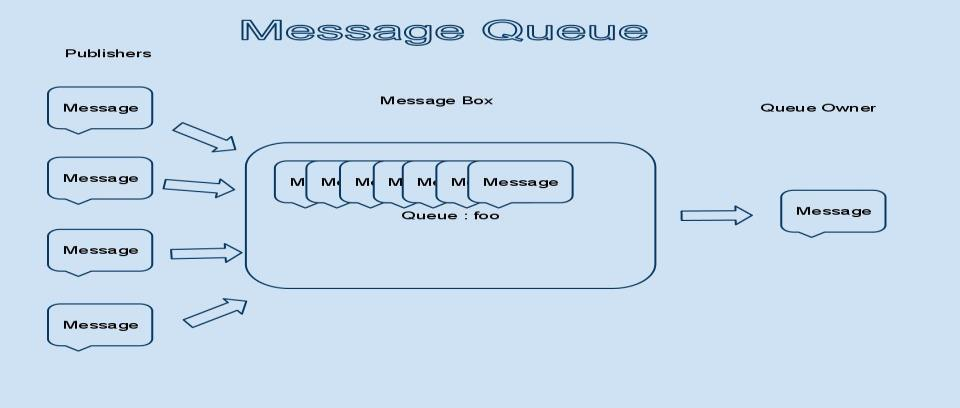
\includegraphics[width=\linewidth]{%
    diagrams/message_queue.png}
  \caption{Scheme of a message queue}
\end{figure}
% }}}

\subsection{RabbitMQ}
\label{s_rabbitmq}
\index{RabbitMQ}

% Introduction {{{
\begin{figure}[H]
  \centering
  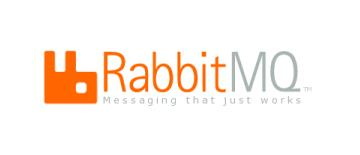
\includegraphics[width=\linewidth/2]{%
    diagrams/rabbitmq_logo.png}
  \caption{RabbitMQ Logo}
\end{figure}

For our project we used RabbitMQ as our messsage broker.

RabbitMQ is an open source message broker software
(sometimes called message-oriented middleware) that
originally implemented the Advanced Message Queuing
Protocol(AMQP) and has since been extended with a plug-in
architecture to support Streaming Text Oriented Messaging
Protocol (STOMP), Message Queuing Telemetry Transport
(MQTT), and other protocols.\cite{amjad22}

The RabbitMQ server program is written in the Erlang
programming language and is built on the Open Telecom
Platform framework for clustering and failover. Client
libraries to interact with the broker are available for all
major programming languages.\cite{amjad23}
% }}}

% Small glance on the history of RabbitMQ {{{
\subsubsection{Small glance on the history of RabbitMQ}

Rabbit Technologies Ltd., originally developed RabbitMQ.
Rabbit Technologies started as a joint venture between
LShift and CohesiveFT in 2007\cite{amjad24}, and was
acquired in April 2010 by SpringSource, a division of
VMware.\cite{amjad25} The project became part of Pivotal
Software in May 2013.\cite{amjad26}

% }}}
